\documentclass[12pt,oneside]{book}
\usepackage{times,mathptmx}
\usepackage[pdftex]{graphicx}
\usepackage{calc}
\usepackage{tabularx,ragged2e,booktabs,caption,subcaption}
\usepackage{array}
\newcolumntype{L}[1]{>{\raggedright\let\newline\\\arraybackslash\hspace{0pt}}m{#1}}
\newcolumntype{C}[1]{>{\centering\let\newline\\\arraybackslash\hspace{0pt}}m{#1}}
\newcolumntype{R}[1]{>{\raggedleft\let\newline\\\arraybackslash\hspace{0pt}}m{#1}}
\usepackage{multirow}
\usepackage{multicol}
\usepackage{tocloft}
\usepackage{xcolor}
\usepackage{color,soul}
\usepackage{amsmath}
\definecolor{linknavy}{rgb}{0,0,0.50196}
\definecolor{linkred}{rgb}{1,0,0}
\definecolor{linkblue}{rgb}{0,0,1}
\definecolor{darkorange}{rgb}{0.81,0.52,0}
\definecolor{fc_orange}{rgb}{0.94,0.59,0.14}
\definecolor{brown}{rgb}{0.56,0.36,0}
\definecolor{fc_blue}{rgb}{0.27,.36,0.48}
\usepackage{float}
\usepackage{graphpap}
\usepackage{rotating}
\usepackage{graphicx}
\usepackage{geometry}
\usepackage{relsize}
\usepackage{ltablex}
\usepackage{longtable}
\usepackage{lscape}
\usepackage{amssymb}
\usepackage{makeidx} % Create index at end of document
\usepackage[nottoc,notlof,notlot]{tocbibind} % Put the bibliography and index in the ToC
\usepackage{lastpage} % Automatic last page number reference.
\usepackage[T1]{fontenc}
\usepackage{enumerate}
\usepackage{upquote}
\usepackage{moreverb}
\usepackage{xfrac}
\usepackage{cite}
\usepackage{tikz}
% \usepackage{subfig}
% \usepackage{caption}
\usepackage[toc,page]{appendix}
\usepackage{notoccite}
\usepackage{placeins}

\usepackage{titlesec}
\titleformat{\chapter}[hang] 
{\color{fc_blue}\normalfont\huge\bfseries}{\chaptertitlename\ \thechapter}{1em}{}[\titlerule]
\titlespacing*{\chapter}{0pt}{-30pt}{20pt}

\titleformat*{\section}{\normalfont\Large\bfseries\color{fc_blue}}
\titleformat*{\subsection}{\normalfont\large\bfseries\color{fc_blue}}

\newcommand{\nopart}{\expandafter\def\csname Parent-1\endcsname{}} % To fix table of contents in pdf.

\usepackage{siunitx}
\sisetup{
    detect-all = true,
    input-decimal-markers = {.},
    input-ignore = {,},
    inter-unit-product = \ensuremath{{}\cdot{}},
    multi-part-units = repeat,
    number-unit-product = \text{~},
    per-mode = fraction,
    separate-uncertainty = true,
}

\usepackage{listings}
\usepackage{textcomp}
\definecolor{lbcolor}{rgb}{0.96,0.96,0.96}

\usepackage[pdftex,
        colorlinks=true,
        urlcolor=fc_orange,     % \href{...}{...} external (URL)
        citecolor=fc_orange,     % citation number colors
        linkcolor=fc_orange,    % \ref{...} and \pageref{...}
        pdfproducer={pdflatex},
        pdfpagemode=UseNone,
        bookmarksopen=true,
        plainpages=false,
        verbose]{hyperref}

\renewcommand{\cftchapfont}{\hypersetup{linkcolor=fc_blue}}
\renewcommand{\cftsecfont}{\hypersetup{linkcolor=black}}
\renewcommand{\cftsubsecfont}{\hypersetup{linkcolor=black}}
\renewcommand{\cftsubsubsecfont}{\hypersetup{linkcolor=black}}


\setlength{\textwidth}{6.5in}
\setlength{\textheight}{9.0in}
\setlength{\topmargin}{0.in}
\setlength{\headheight}{0.pt}
\setlength{\headsep}{0.in}
\setlength{\parindent}{0.0in}
\setlength{\itemindent}{0.25in}
\setlength{\oddsidemargin}{0.0in}
\setlength{\evensidemargin}{0.0in}
% \setlength{\leftmargini}{\parindent} % Controls the indenting of the "bullets" in a list
\setlength{\cftsecnumwidth}{0.45in}
\setlength{\cftsubsecnumwidth}{0.5in}
\setlength{\cftfignumwidth}{0.45in}
\setlength{\cfttabnumwidth}{0.45in}
\setlength{\parskip}{1em}

% \newcolumntype{L}{>{\centering\arraybackslash}m{4cm}}

\floatstyle{boxed}
\newfloat{notebox}{H}{lon}
\newfloat{warning}{H}{low}

\newenvironment{conditions}
  {\par\vspace{\abovedisplayskip}\noindent\begin{tabular}{>{$}l<{$} @{${}={}$} l}}
  {\end{tabular}\par\vspace{\belowdisplayskip}}


% Rename chapter headings
\renewcommand{\chaptername}{}
\renewcommand{\bibname}{References}

\usepackage{tikz}
\usetikzlibrary{calc}

\usepackage{fancyhdr}
\pagestyle{fancy}
\lhead{}
\rhead{}
\chead{}
\renewcommand{\headrulewidth}{0pt}


% \usepackage{draftwatermark}
% \SetWatermarkText{DRAFT}
% \SetWatermarkScale{1}

\begin{document}
\pagenumbering{gobble}

\bibliographystyle{unsrt}
%\pagestyle{empty}

\frontmatter

\begin{minipage}{1.0\textwidth}
\pagecolor{fc_blue}
\pagenumbering{gobble}

\vspace{1cm}
\centering

\includegraphics[width=2.5in]{Figures/firecares-header-logo_2}
\noindent\makebox[\linewidth]{\color{white}\rule{.5\paperwidth}{0.6pt}}

\Huge \color{fc_orange} User and Implementation Guide \\

\vspace{0.5cm}

\large{\color{white} Version: 1.5  \hspace{1cm} Compilation Date: \today \\}

\vspace{4cm}

{\Large \em \color{fc_orange}Analyze how fire department resources \\
are deployed to match a community's risks. \\
}
\end{minipage}


\frontmatter
\pagecolor{white}

% \newpage
% \hspace{5in}
% \newpage

\pagestyle{fancy}{
\fancyhf{}
\fancyhead[]{%
   \begin{tikzpicture}[overlay, remember picture]%
   \fill[fc_blue] (current page.north west) rectangle ($(current page.north east)+(0,-.5in)$);
   \node[anchor=north west, text=white, font=\Large\scshape, minimum size=1in, inner xsep=5mm] at (current page.north west) {};
   \end{tikzpicture}
}
\fancyfoot[C]{
   \begin{tikzpicture}[overlay, remember picture]%
   \fill[fc_orange] (current page.south west) rectangle ($(current page.south east)+(0,.5in)$);
   \node[anchor=south west, text=black, minimum size=.5in] at (current page.south west) {\thepage};
   \end{tikzpicture}
}}


\fancypagestyle{plain}{
\fancyhf{}%
% \fancyfoot[C]{\thepage\ of \pageref{LastPage}}%
\fancyhead[]{
   \begin{tikzpicture}[overlay, remember picture]% 
   \fill[fc_blue] (current page.north west) rectangle ($(current page.north east)+(0,-.5in)$);
   \node[anchor=north west, text=white, font=\Large\scshape, minimum size=1in, inner xsep=5mm] at (current page.north west) {};
   \end{tikzpicture}
}
\fancyfoot[C]{
   \begin{tikzpicture}[overlay, remember picture]%
   \fill[fc_orange] (current page.south west) rectangle ($(current page.south east)+(0,.5in)$);
   \node[anchor=south west, text=black, minimum size=.5in] at (current page.south west) {\thepage};
   \end{tikzpicture}
}}


\pagenumbering{roman}

\newpage

\cleardoublepage


% \phantomsection

\renewcommand*\contentsname{\color{fc_blue}Contents}
\tableofcontents

\hypersetup{ 
    linkcolor=fc_orange,         % moved after \tableofcontents
    filecolor=fc_orange,      % 
    urlcolor=fc_orange,           %
}    

\newpage
\mainmatter

\chapter{Introduction to FireCARES}

A fire department's relationship with data and performance should be seen as a continuum. Statements regarding a department's need to have ``good data'' and ``good performance'' are numerous. However, these statements are not the same thing. The beginning of the quality performance continuum is for a department to have ``good data.'' Good data is defined as data that are based on factual incidents, reported accurately, and can be accessed and manipulated easily. It can take a department a long time to work on their data but it is important to recognize their ability to quantify impact before instituting change. Without good data there is no assurance that improvement efforts actually work.

Once a department has improved their data quality, they can begin working on having ``good performance.'' Good performance is the end of the quality improvement continuum. For example, improving fire station layouts to reduce turnout time, working with the communications center to streamline call processing, conducting targeted staff training, investing in community risk reduction efforts, and deploying additional/alternate resources within a jurisdiction are all ways to improve performance. 
A knee jerk reaction to observing a given performance metric for a department may be to say that ``the metric is wrong.'' However, in determining the root cause, it is important to distinguish whether the data used in the calculations are wrong or the performance itself is poor.  

\href{https://firecares.org}{FireCARES} is designed to analyze how fire department resources are deployed to match community risks. Local government decision makers often alter fire department resources faster than fire service leaders can evaluate the potential impact. These decisions can leave a community without sufficient resources to respond to emergency calls safely, efficiently, and effectively. These decisions can have even greater impact on vulnerable populations including the elderly, young children, and people with disabilities. FireCARES - Community Assessment, Response Evaluation System - is an analytical system designed to evaluate community risk and fire department operational performance using national data layers in a geographic-based system. The FireCARES project provides fire departments the ability to add a technical basis to what has historically been an anecdotal discussion regarding community hazards and risks as well as the impact of changes to fire department resource levels. FireCARES includes more than a decade of research on structure fires and related injuries and death, as well as building footprints, housing and mobile home units, public health and census data, and locations of vulnerable populations.

The goal of the project, which is funded by DHS/FEMA's Assistance to Firefighter's Grants is to aggregate national and local data to provide answers that both public and fire service leaders have not previously had. To accomplish this task, FireCARES provides three scores for each community dependent on the available data: the Community Risk Score, the Fire Department Performance Score, and the Safe Grade.

\chapter{FireCARES Scores}


To assess risk and fire department performance, it was important to establish filters that define comparisons between departments. A small rural department does not face the same risks or have the same resources as a major metropolitan department. Therefore, it would be unfair to both departments for that comparison to occur. Currently, department comparison groups are determined by NFPA geographical region (Northeast, South, Midwest, and West) and population protected class (there are 10 NFPA population protected classes).

\section{Community Risk}

The community risk score was developed as a function of the socio-demographic and geographic characteristics of the locations (census tracts) of reported structure fires over a seven year period (2008-2014) according to available National Fire Incident Reporting System (NFIRS) data. The community risk score is determined by assessing variables that are known to contribute to fire like building materials, population demographics, and smokers. The socio-demographic attributes include:

\begin{itemize}
\item Population characteristics (e.g., size category of the department, population, number of males, age group counts, race counts)
\item Housing characteristics (e.g., total housing units, total vacancies, size of home, number of renters, age of units)
\item Household characteristics (e.g., median household income, social vulnerability index)
\item Geographic region
\end{itemize}

Community risk assessment scores are calculated for the community as a whole. The community risk scores actually contain three separate scores 

\begin{itemize}
\item Risk of Fire
\item Risk of Fire Spread
\item Risk of Death and Injury
\end{itemize}

Once scores are determined for each jurisdiction, the jurisdictions are grouped with like areas and populations.  The grouping then allows a comparison of community risk scores between each jurisdiction.  The jurisdictions in the like group are then ranked into the top 25\%, the medium 50\%, and the lower 25\% in their group. Figure~\ref{fig:risk} shows how the community risk scores are displayed.

\begin{figure}[ht!]
\centering
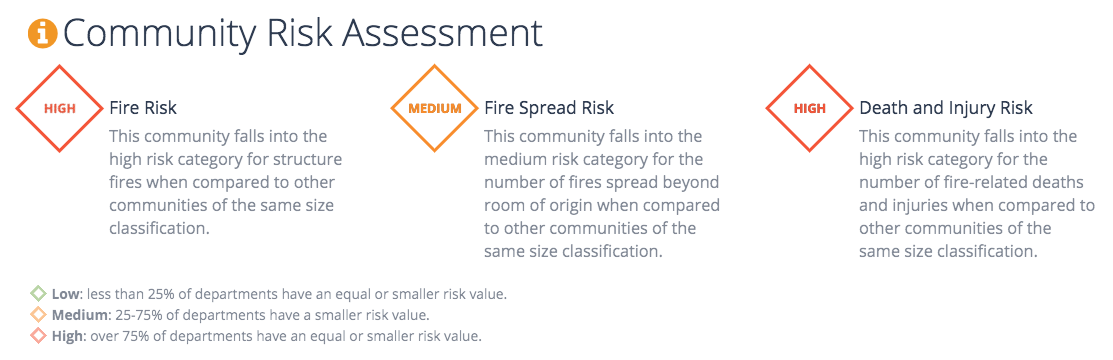
\includegraphics[width=.9\columnwidth]{Figures/risk}
\caption{Community Risk Scores}
\label{fig:risk}
\end{figure}

For this example department, the community risk would read like ``the community this department protects is at a high risk for the occurrence of fire.'' That means the community falls into the bottom quartile (riskiest 25\%) compared to similar jurisdictions.

\section{Fire Department Performance Score}

The goal of the fire department performance score is to assess how well a fire department performs compared to the ``standardized'' version of itself. One component of this metric is the structure fire spread category from NFIRS. This category provides information which quantifies the fire spread in a structure from confined to object of origin through spread beyond structure of origin. There are five categories defined in NFIRS, but for this analysis the data are collapsed into three categories: room of origin (lumping object and room together), floor of origin (lumping floor and structure together), and beyond structure of origin. The resulting distribution (count of fires in each of the three bins) of fire spread is the basis for comparison for developing the performance score.

The second component of this score is the model that defines how the fire department would perform if it were acting as a standard, idealized version of itself. The concept is that there exists a theoretical version of every fire department where all responses meet or exceed the national standards governing department performance. Essentially, a fire department responding to a fire must complete a series of tasks before they can put water on the fire. For purposes of this model these tasks are broken up as follows:

\begin{itemize}
\item Time to alarm - Time required before the fire is noticed, and some form of action is taken [NIST TN 1661~\cite{NIST:Residential}, NIST TN 1797~\cite{NIST:HighRise}]
\item Time to dispatch - Time required for dispatch operator to obtain enough information regarding the fire and location to issue a dispatch [NFPA 1710/1720~\cite{nfpa_1710,nfpa_1720}]
\item Time to turnout - Time required for firefighter turnout [NFPA 1710/1720~\cite{nfpa_1710,nfpa_1720}]
\item Time to arrival - Transit time required for engine between station and fire location [NFPA 1710/1720~\cite{nfpa_1710,nfpa_1720}, GIS]
\item Time to ascend - Transit time required for firefighters to ascend to the staging floor for fires in buildings. Data for ascent was gathered from timed 27-story climb experiments with 35 firefighters of varying age, height, weight, and gender. Note this parameter is only enacted when staging would occur above ground level.
\item Time to suppress - Time required for firefighters on-scene to put water onto fire (includes size-up, hose connection, etc.) [NIST TN 1661~\cite{NIST:Residential}, NIST TN 1797~\cite{NIST:HighRise}]
\end{itemize}

When water is put onto a fire, the idealized fire is assumed to have reached the peak size. The growth time for the fire is equivalent to the sum of the tasks the fire department must perform to suppress the fire. This time to suppression is coupled to a simple exponential area damage growth model which is consistent with fire statistics literature. A distribution of fire spread is generated using the same three NFIRS bins discussed above, based on the modeled area of fire damage at the suppression time. Distributions of the room and building sizes are estimated from the American Housing Survey's (AHS) national survey of residential homes. Where available, it is possible to use the AHS metropolitan statistical areas to refine room and building distributions for larger metropolitan areas.

The concept is that there exists an average time correction for all fire department structure fire responses routed through the idealized fire department model that ``corrects'' the fire damage outcomes expected from national standards to the particular outcomes observed by a given fire department. This average correction time is known as the fire department performance score. Figure~\ref{fig:perform} shows the performance score for an example department. The number in center of the dial is performance, or average time in seconds the department is over it's idealized performance. The numbers on the left and right side of the dial are the minimum and maximum performance scores for the departments in the same grouping (location and size).

\begin{figure}[ht!]
\centering
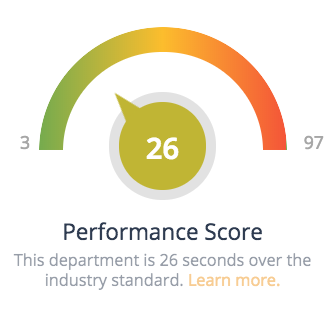
\includegraphics[width=.5\columnwidth]{Figures/performance_score}
\caption{Performance Score}
\label{fig:perform}
\end{figure}

The gauge indicates whether the performance score is good, fair, or poor. First the colors green, yellow, and red indicate good (top 25\%), fair (middle 50\%) and poor (bottom 25\%) quartiles. This gauge compares the department to other like departments and as you can see this department falls in the green quartile. 

\FloatBarrier

\section{Safe Grade}

A community's set of safe grades represent an assessment of the number of fires, of fire spread, and of civilian and firefighter injury or death based on how well the Fire Department resources (performance score) match the level of risks within the community (risk score). Therefore, given your community risk assessment score and given your Fire Department's historic response capabilities and performance, the safe grade is either good, fair, or poor depending on how well you match resources deployed to the risks in the community. There are 3 safe grade comparison categories:

\begin{itemize}
\item Performance based on number of fires
\item Performance based on fire spread
\item Performance based on injury and death
\end{itemize}

For each category, your department is compared against similar departments and based on the risk group (low, medium, high) the community falls within for the respective category (see above). Then based on your performance score relative to those other departments, your safe grade is either good, fair, or poor. A {\it good}, safe grade represents the top 25\%, a {\it fair} safe grade represents the median 50\%, and a {\it poor} safe grade represents the bottom 25\%.

All three scores can be filtered by the hazard level of structures: low, medium, and high as defined by NFPA. This is filterable on the department landing page by clicking on the the hazard level bar above the performance score. 

\chapter{Using FireCARES.org}

When you arrive at \href{https://firecares.org}{FireCARES.org}, begin by typing a fire department name or municipality in the search bar (Figure~\ref{fig:homepage}). 

\begin{figure}[ht!]
\centering
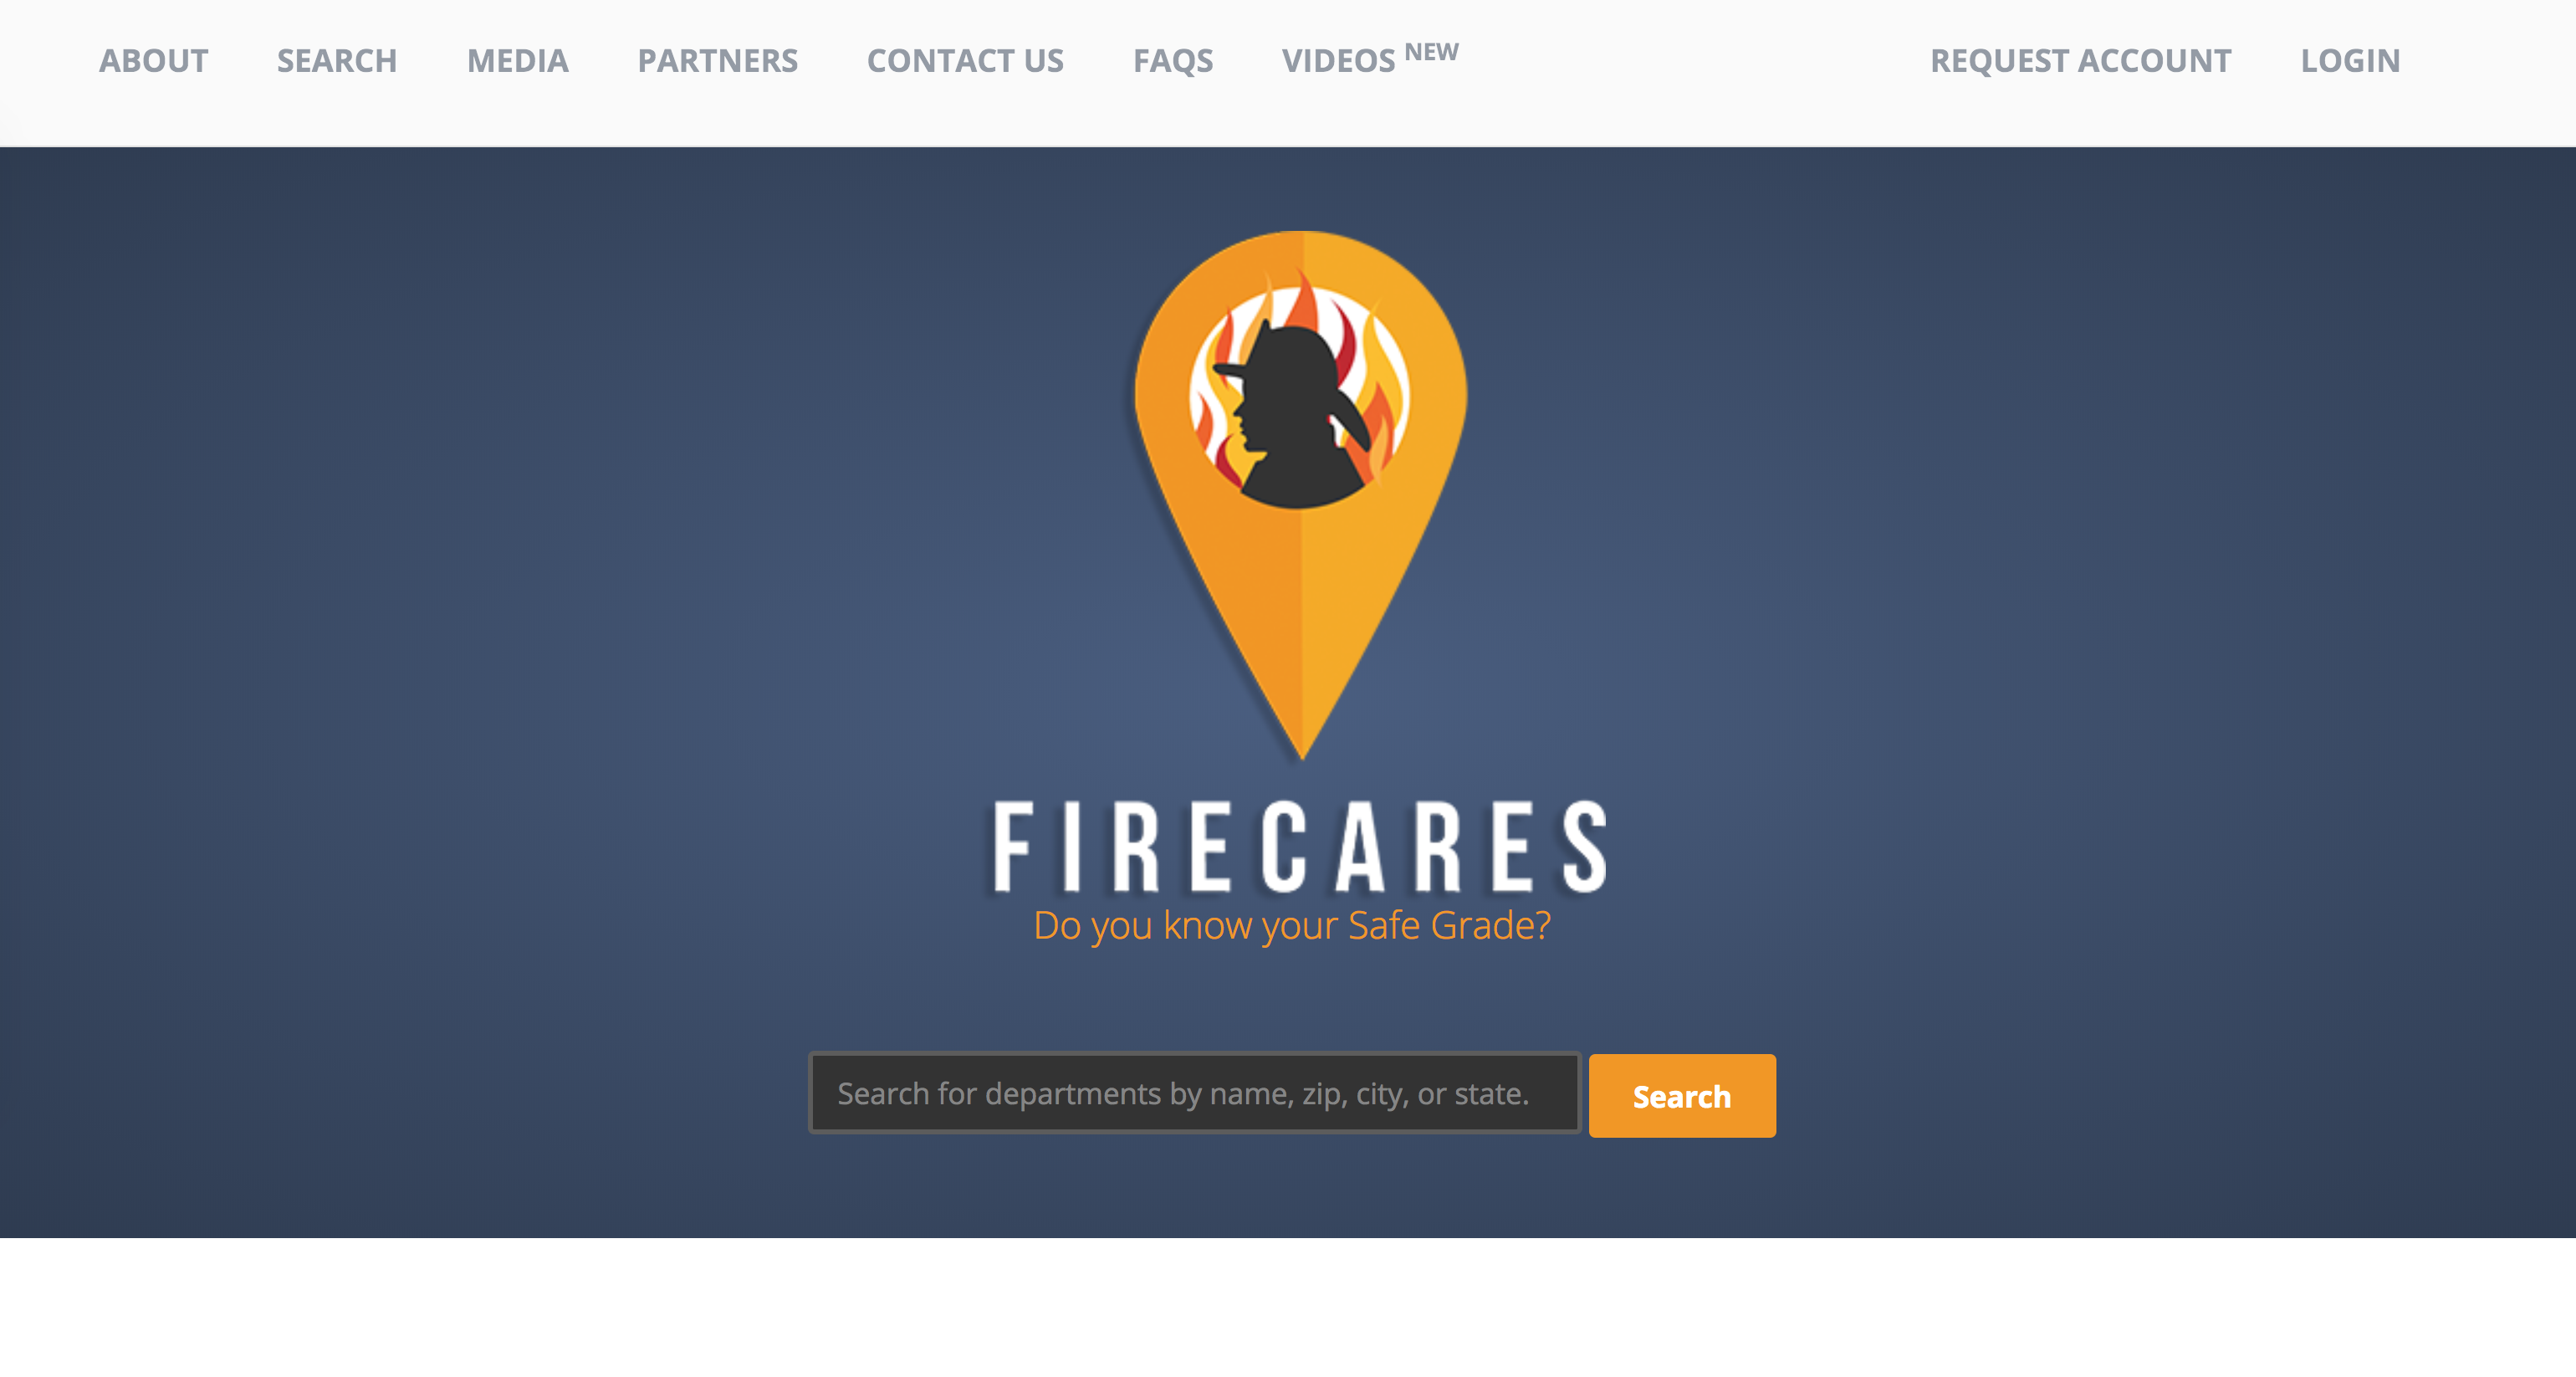
\includegraphics[width=.9\columnwidth]{Figures/homepage}
\caption{FireCARES Homepage}
\label{fig:homepage}
\end{figure}

If you know the department you are looking for, enter it in the search bar and click the dialog box. If you leave the bar blank, results will be returned for all of the departments in FireCARES. As you can see in Figure~\ref{fig:search}, there are 27k+ fire departments in FireCARES. The goal is to have a landing page for every fire department, anywhere in the United States. On the left hand side of the Figure~\ref{fig:search}, you can see that search results can be filtered by department name, FDID, state, geographical region, performance score or protected population. You can also search through all of the field by entering your query in the top box.

\begin{figure}[ht!]
\centering
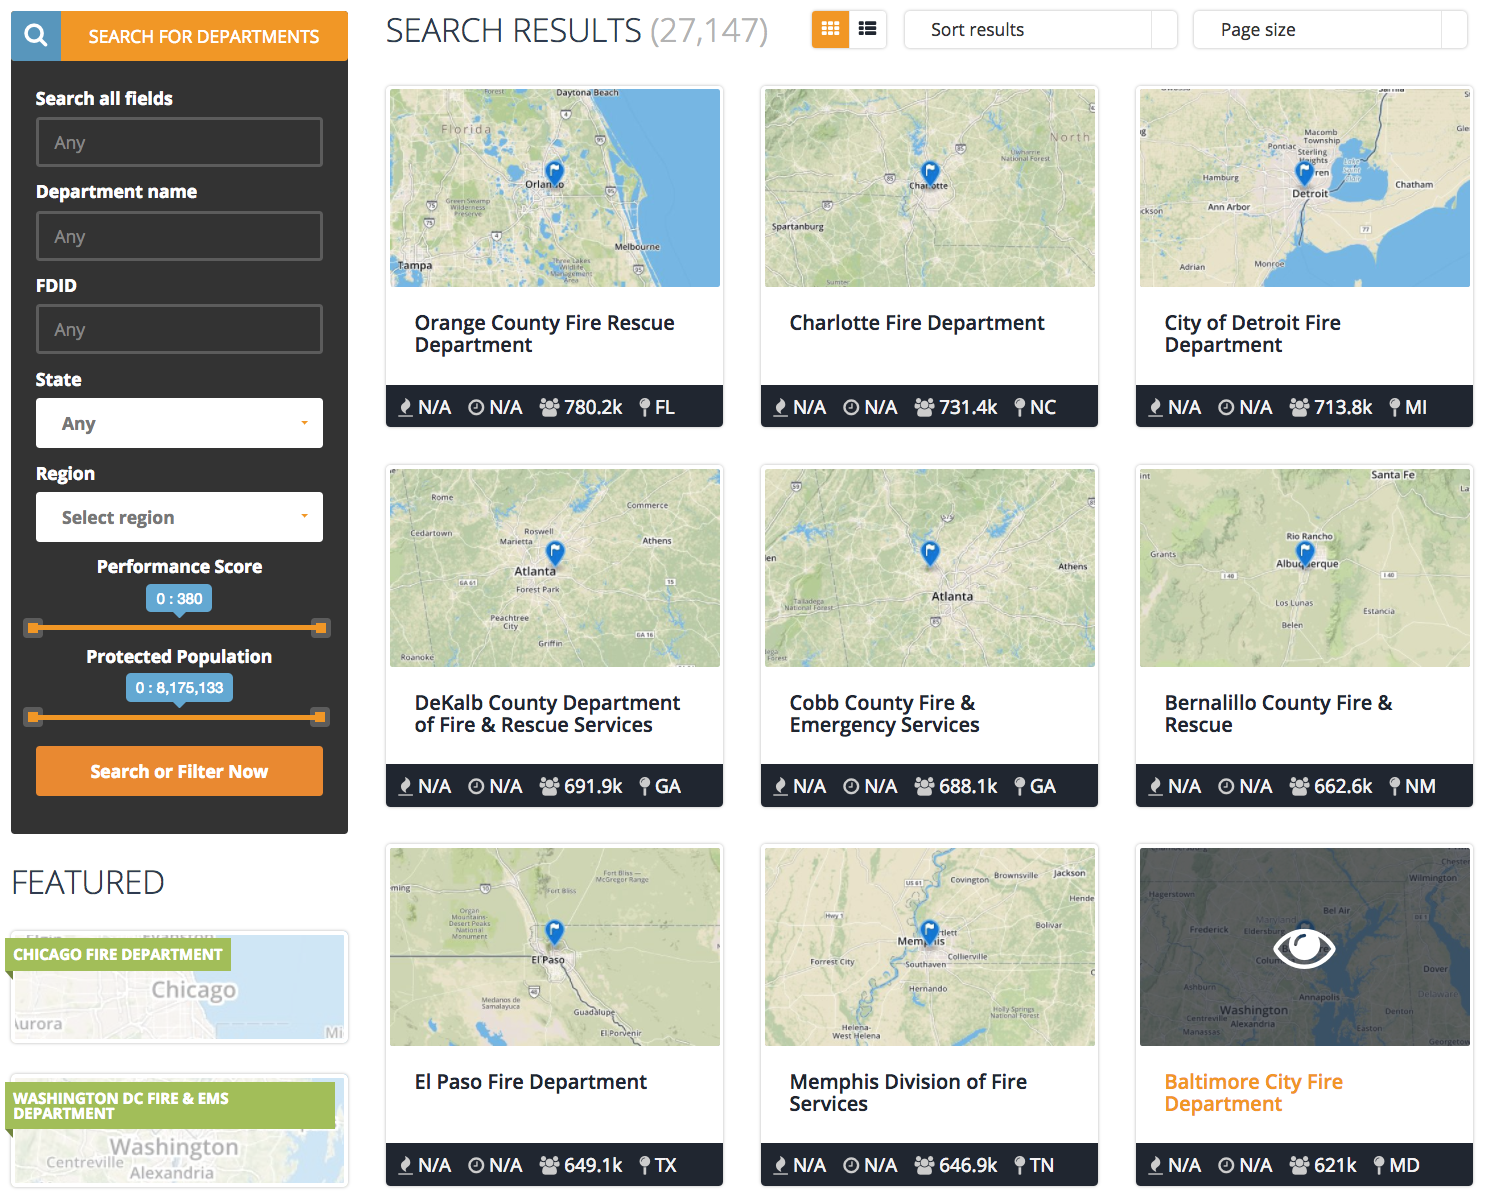
\includegraphics[width=.9\columnwidth]{Figures/search_results}
\caption{FireCARES Search Results}
\label{fig:search}
\end{figure}

\FloatBarrier

Clicking on a department's map image or name will take you to that departments landing page. Note that if you are not logged in, the department page will look like Figure~\ref{fig:department_page_nologin}. For the three scores generated by FireCARES, only the community risk scores are available without login. The fire department performance score and safe grades are only available upon login and will appear `gray-ed out'.

\begin{figure}[ht!]
\centering
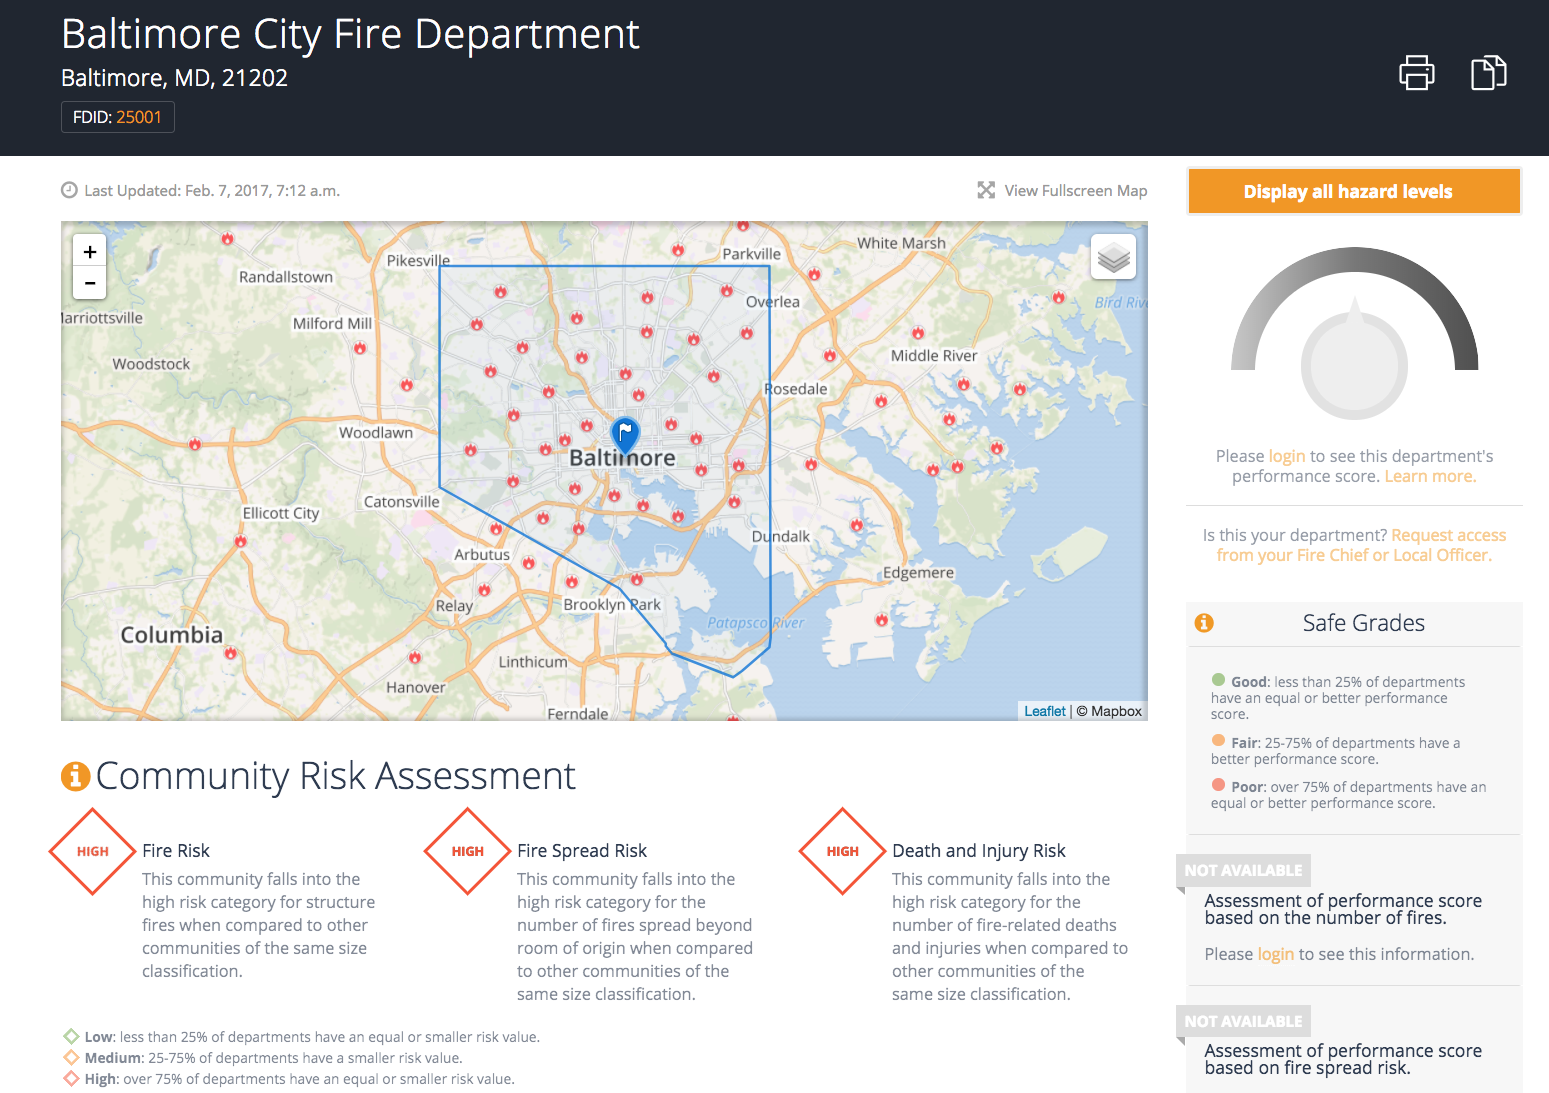
\includegraphics[width=.9\columnwidth]{Figures/department_page_logout}
\caption{FireCARES department landing page without login}
\label{fig:department_page_nologin}
\end{figure}

\FloatBarrier

\section{Logging In}

Login credentials will be granted to the fire chief, the local union president (when applicable) and/or their designees. If you are an IAFF president or an IAFF officer, you can login using your IMIS credentials. If you an IAFC member, you can login using your Helix credentials. The left image in Figure~\ref{fig:login} shows the FireCARES login dialog box.

\begin{figure}[ht!]
\centering
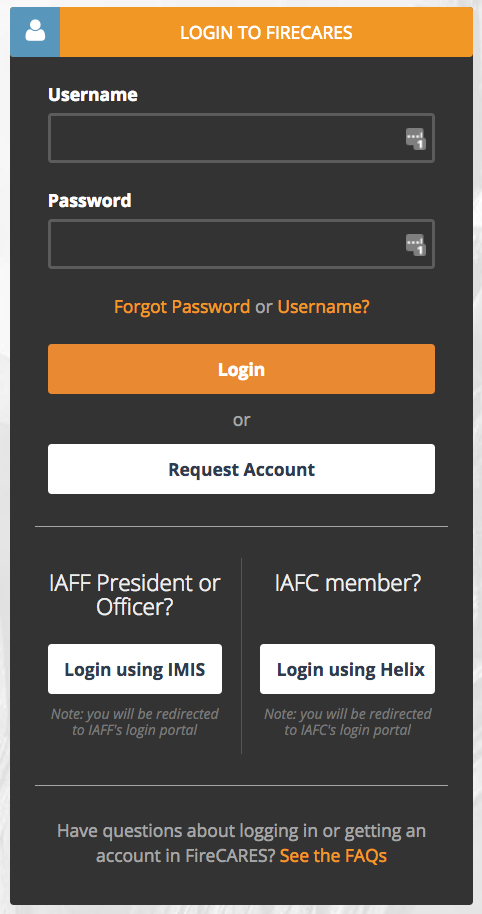
\includegraphics[width=.45\columnwidth]{Figures/login}
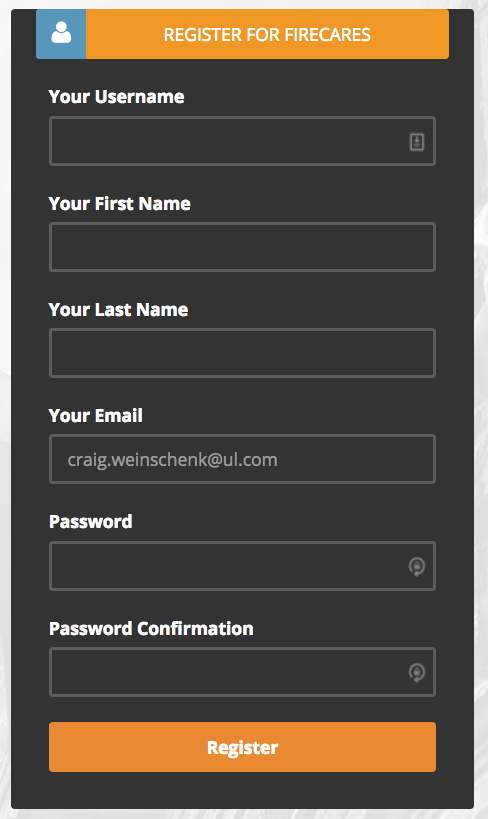
\includegraphics[width=.45\columnwidth]{Figures/login2}
\caption{FireCARES Login Dialog (left) and Registration Dialog (right)}
\label{fig:login}
\end{figure}

If you do not have an account, are not sure if you have an account, or IMIS/Helix do not apply, click on the request account box. Enter your email and click the `Check registration' box. If you do have an account, a request for an account from that email address will be made. If an account associated with that email exists, then you will be redirected back to the login page. 

Once an email has been approved, the user will be directed to the registration screen. This dialog box will require you to enter your name, email address, login username and password.  Following entry of these attributes, the user will click the ``Register'' icon (see right image in Figure~\ref{fig:login}). Users will then be able to log into FireCARES.

An authenticated user can provide login authority to others in their department as they deem necessary and appropriate, but must keep a record of those authorized. To provide login authority, the Chief and/or local union president will provide a list of eligible emails to FireCARES administration.  Upon receipt, logins will be created for each email provided.

To minimize logins being shared, a robust password should be implemented upon registration. Changing passwords on 90 day cycles is strongly encouraged but will not initially be required.

\clearpage

\section{Department Details}

Once logged in, users will now see the two additional scores (performance score and safe grades) as well as other features for the department. From Figure~\ref{fig:department_page}, you can see that the performance score and safe grades are active down the right side of the page along with with the publicly available community risk score below the map.

\begin{figure}[ht!]
\centering
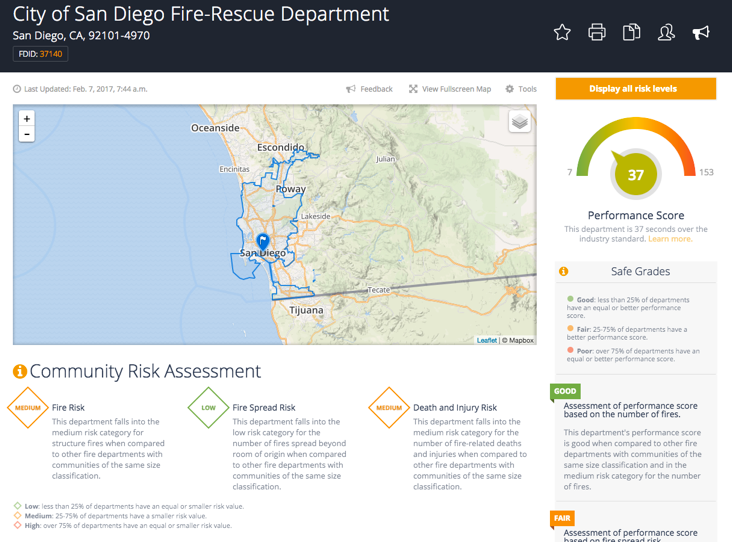
\includegraphics[width=.9\columnwidth]{Figures/department_page}
\caption{FireCARES department landing page}
\label{fig:department_page}
\end{figure}

When viewing your department's page, the first item to check is to ensure that your department's jurisdictional boundary (the blue outline in Figure~\ref{fig:department_page}) is present and accurate.  From your boundary, both your protected area and protected population are calculated (cf. Figure~\ref{fig:description}). The protected population is determined using US Census data. If you notice differences in your population, your protected area, or if your boundary has changed, please send an email to: \href{mailto:boundaries@firecares.org}{Contact Us: Boundaries}. Be sure to include your Fire Department Name and FDID as it is specified on \href{https://www.FireCARES.org}{FireCARES.org}. If you send an updated GIS shapefile for your jurisdictional boundary, the preferred projection is WGS84, however we can convert if the existing projection is specified.

\begin{figure}[ht!]
\centering
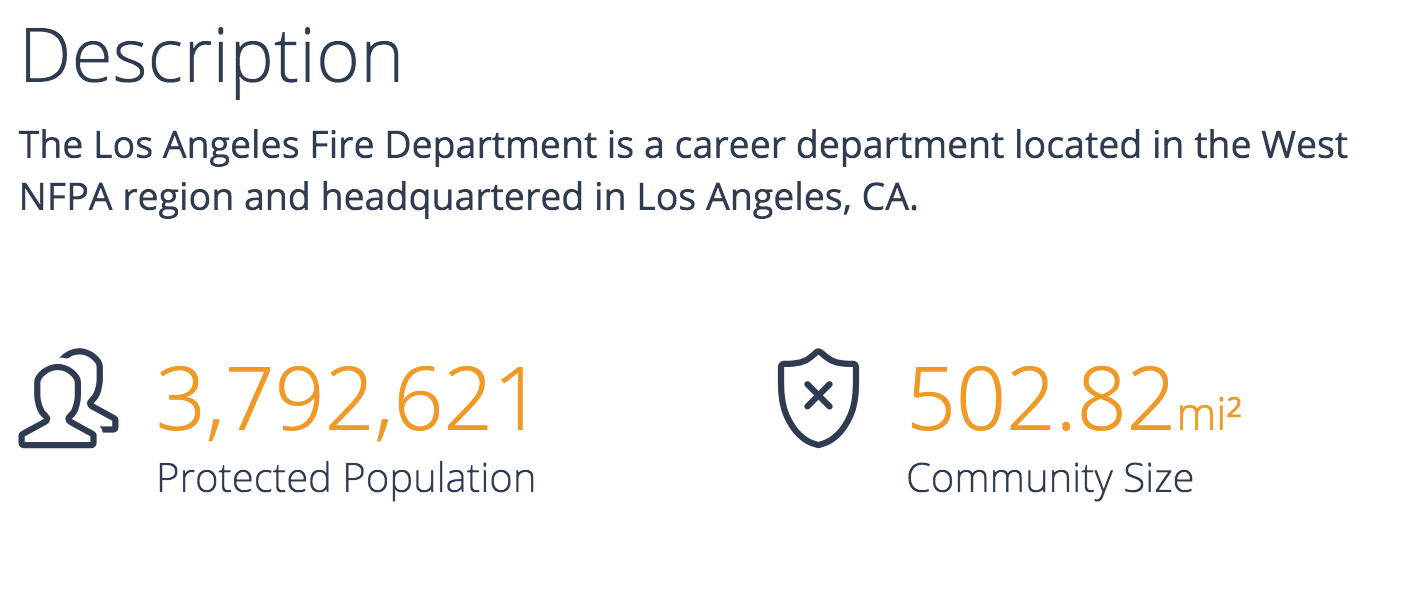
\includegraphics[width=.9\columnwidth]{Figures/description}
\caption{Department protected population and area}
\label{fig:description}
\end{figure}

\FloatBarrier

Additional descriptive features about your department are:

\begin{itemize}
\item Department Type [USFA]
\item NFPA Region [NFPA]
\item FDID [USFA/NFIRS]
\item State 
\item Phone/Fax [USFA Census]
\item Website link
\end{itemize}

as shown in Figure~\ref{fig:description2}.

\begin{figure}[ht!]
\centering
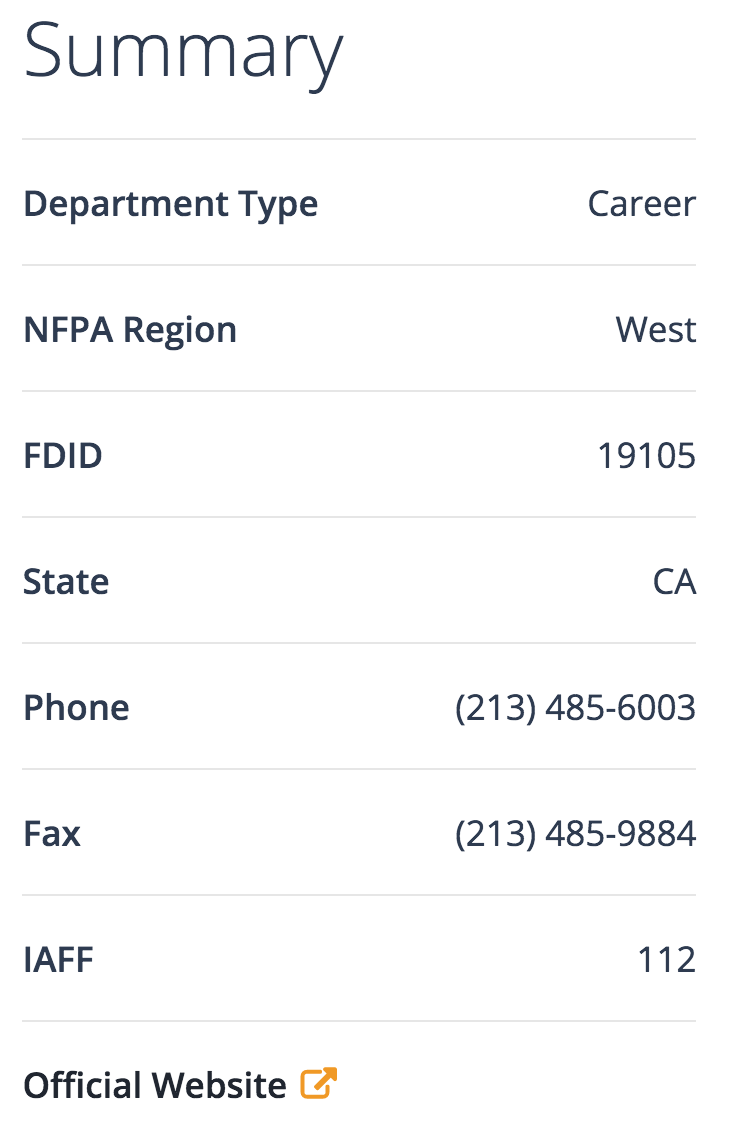
\includegraphics[width=.5\columnwidth]{Figures/description2}
\caption{Department Summary}
\label{fig:description2}
\end{figure}

\FloatBarrier

\section{Annual Structure Fires}

The annual structure fire counts are determined by the data sent by each department to the National Fire Incident Reporting System (NFIRS). In Figure~\ref{fig:structure_fires}, when available, NFIRS data is shown from 2002 to 2014. The middle column represents those fires which were coded as structure fires within the NFIRS system. The right column shows a color bar where the maximum value is the total number of fire calls in NFIRS for that specific calendar year and the black triangle indicates the number of structure fires. This allows users to visualize consistency in data from year to year in both number of fire calls and percentage of structure fires. Note that data is based on the publicly available NFIRS data. If your department would like to send newer NFIRS data, FireCARES can directly ingest NFIRS exchange files. This can be done using the paper icon in the upper right of your department landing page. 

\begin{figure}[ht!]
\centering
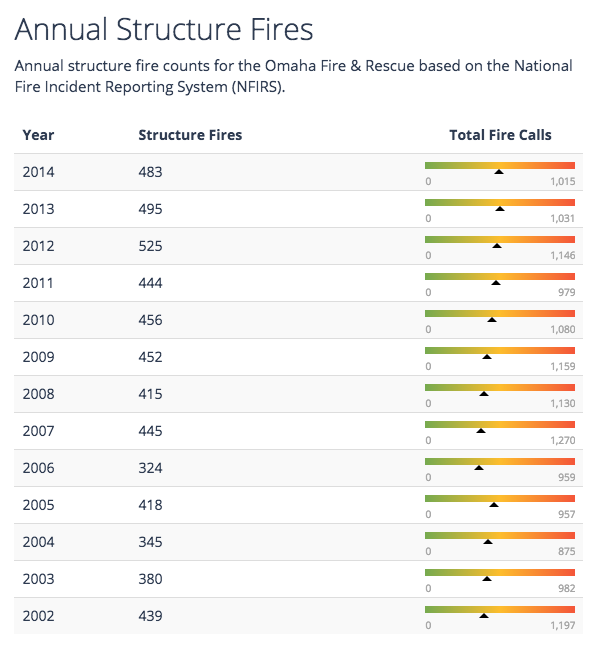
\includegraphics[width=.65\columnwidth]{Figures/structure_fires}
\caption{Annual counts of structure fires (completed structure fire module in NFIRS and total fire calls).}
\label{fig:structure_fires}
\end{figure}

\section{Station Detail Page}

On each department page, the department's list of stations is included, both the station name and address. If there are missing stations, stations that are no longer active, or if the station list is error, either the station name or station address, please send an email to: \href{mailto:boundaries@firecares.org}{Contact Us: Stations}.

Users can also select a particular station from the station list and that station will open into its own landing page. If first due areas have been provided, the stations first due area will also appear. In this view, users can click the GIS layer box (stack of paper icon in the upper right corner of the map) to turn on `Service Area' to see GIS mapping from that station for 4-minute, 6-minute, and 8-minute travel time. All maps are printable using the printer icon at the top of the page. Figure~\ref{fig:response_area} shows an example service area calculation.

\begin{figure}[ht!]
\centering
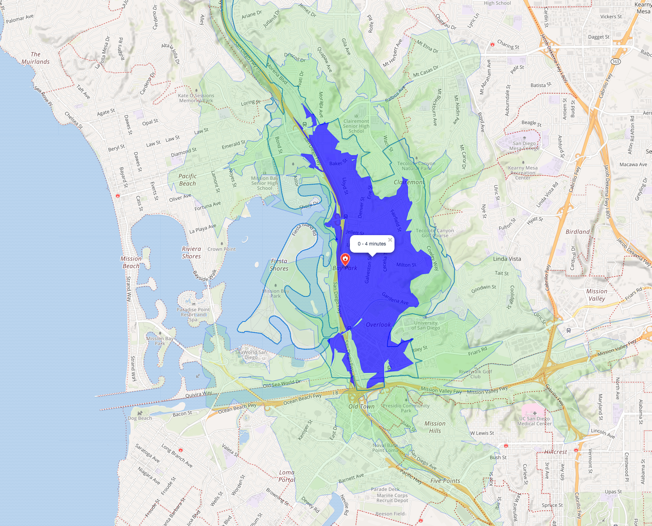
\includegraphics[width=.9\columnwidth]{Figures/response_area}
\caption{GIS based response polygons for 0-4 minute travel times, 4-6 minute travel times, and 6-8 minute travel times.}
\label{fig:response_area}
\end{figure}

\FloatBarrier

In addition to the service area calculations, apparatus and staffing tables can be completed on each station detail page. Departments are requested to complete station tables so that additional GIS features like effective response force (ERF) assembly times by hazard levels, which is coming soon, can be completed. The ERF is calculated by hazard levels. Figure~\ref{fig:staffing} shows an example of the form for entering your staffing data. Users can select an apparatus type, the number of personnel, and whether advanced life support is provided, when applicable. After entering the data, remember to click `Save' before clicking on the `Add Apparatus' tab.

\begin{figure}[ht!]
\centering
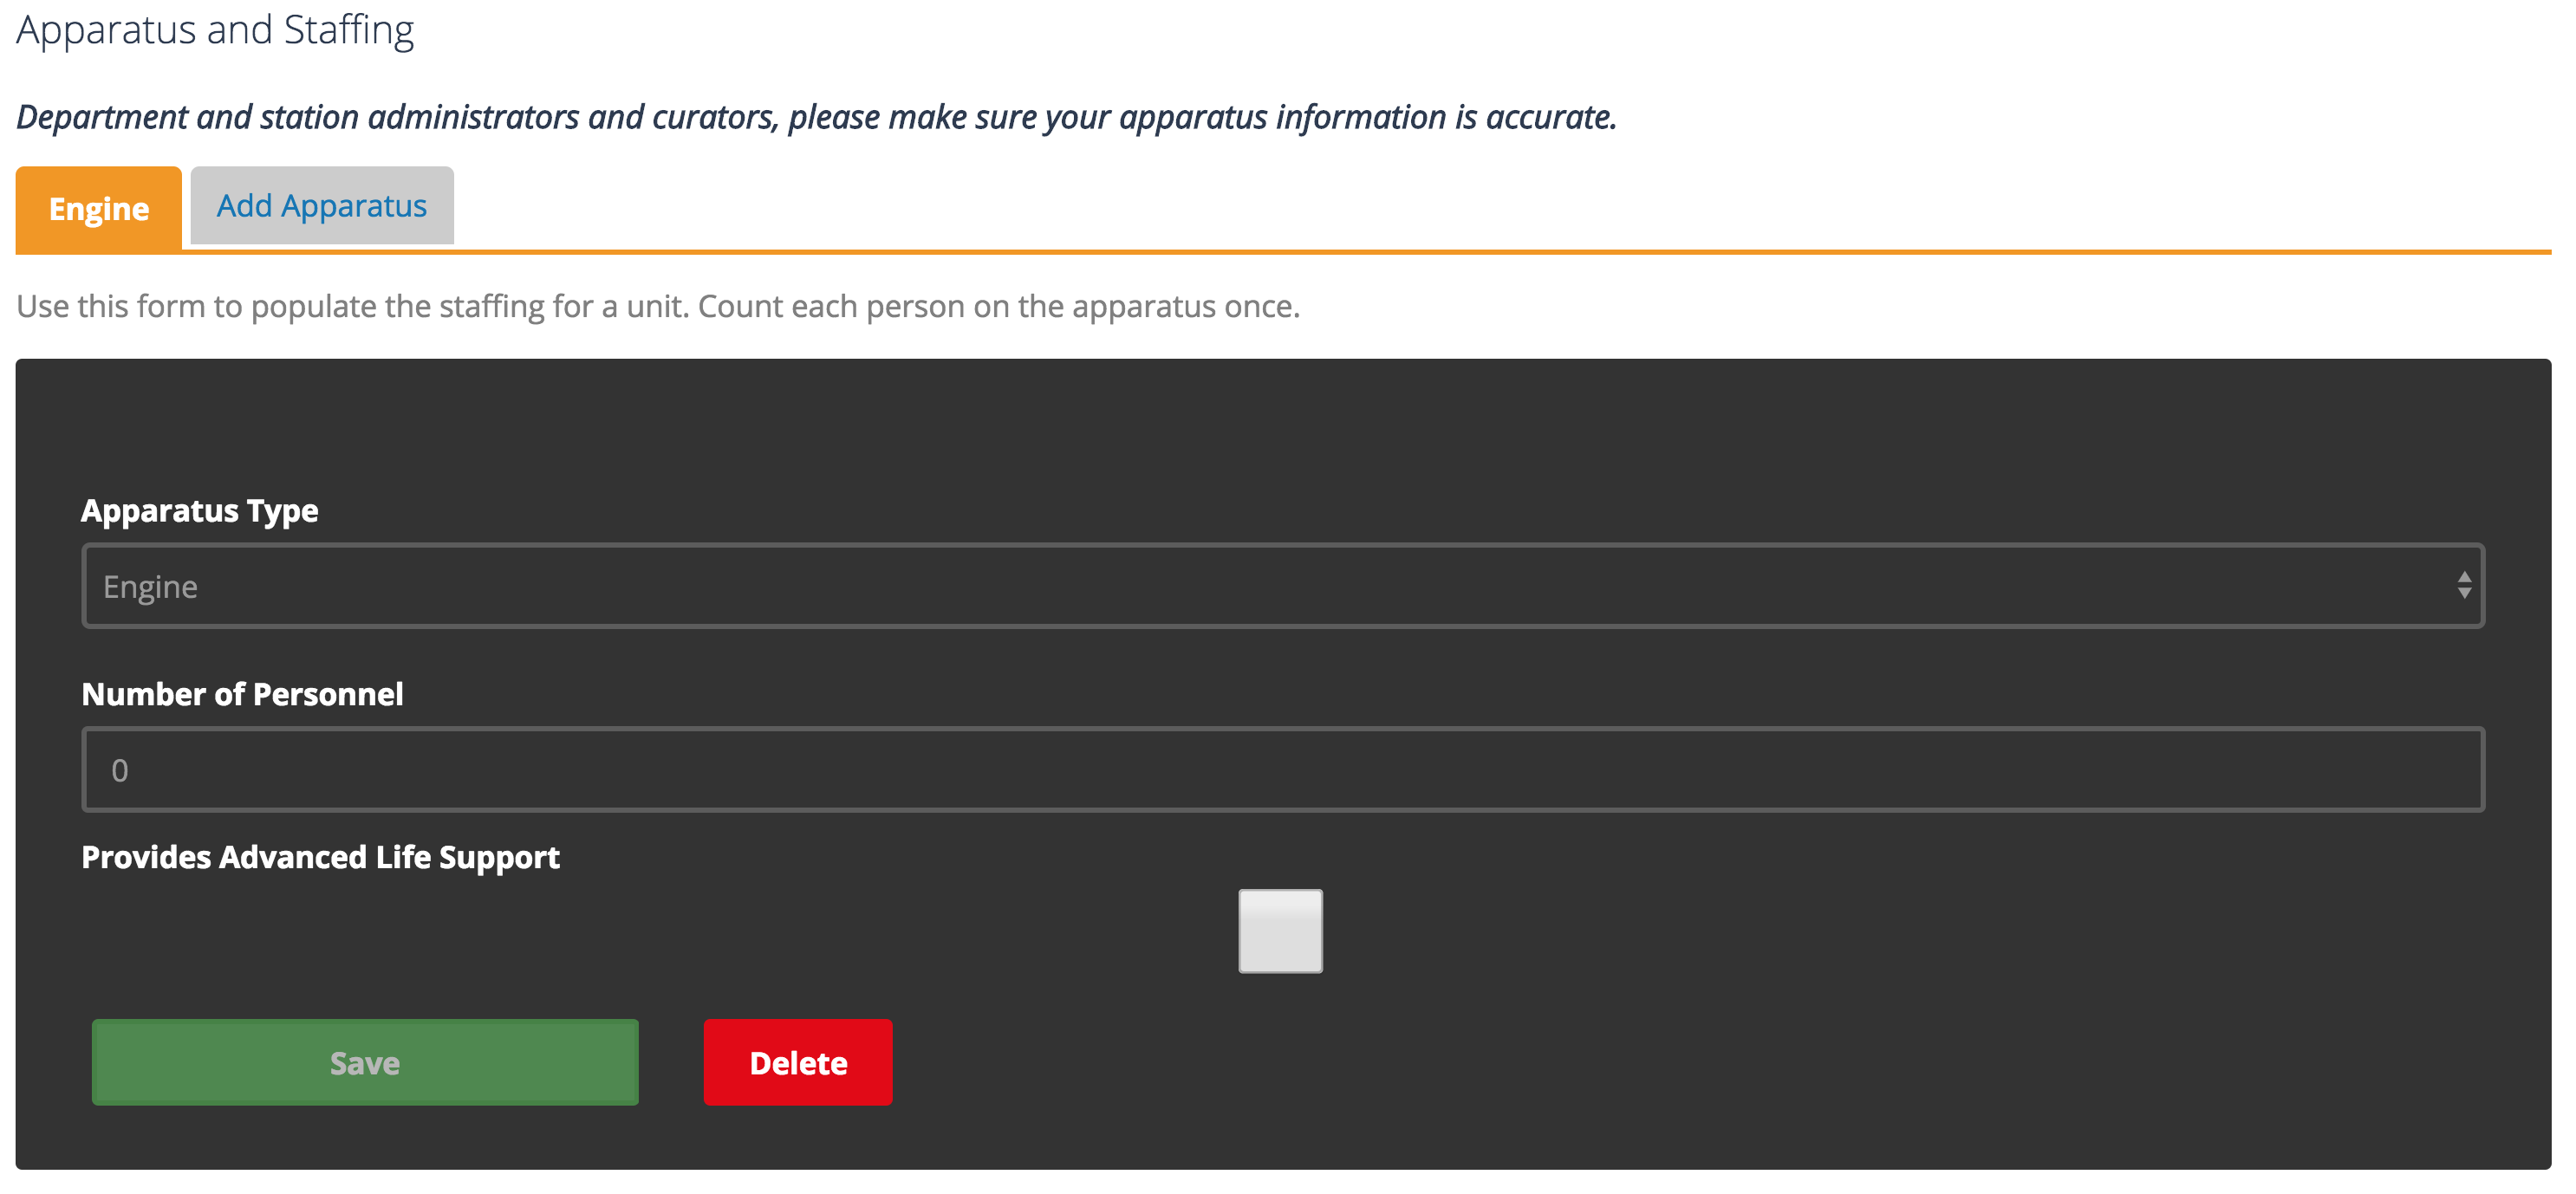
\includegraphics[width=.9\columnwidth]{Figures/staffing}
\caption{Apparatus and Staffing Table}
\label{fig:staffing}
\end{figure}

\FloatBarrier

\section{Interactive Fires Heat Map}

Click the heat map to view more than 12 years of fires that occur in the community. The feature is turned on by hovering over the stack of paper icon in the upper right corner of the map and clicking on the `Fires Heatmap' radio button. Call volume is indicated by green, yellow, and red areas. High call volume is indicated by red areas and low call volume by green. If you zoom in on the map, the coloring will dynamically adjust based on the calls that occurred within the boundaries of the map window. When this feature is turned on, a dashboard will appear below the map (cf. Figure~\ref{fig:interactive_fire_map})

\begin{figure}[ht!]
\centering
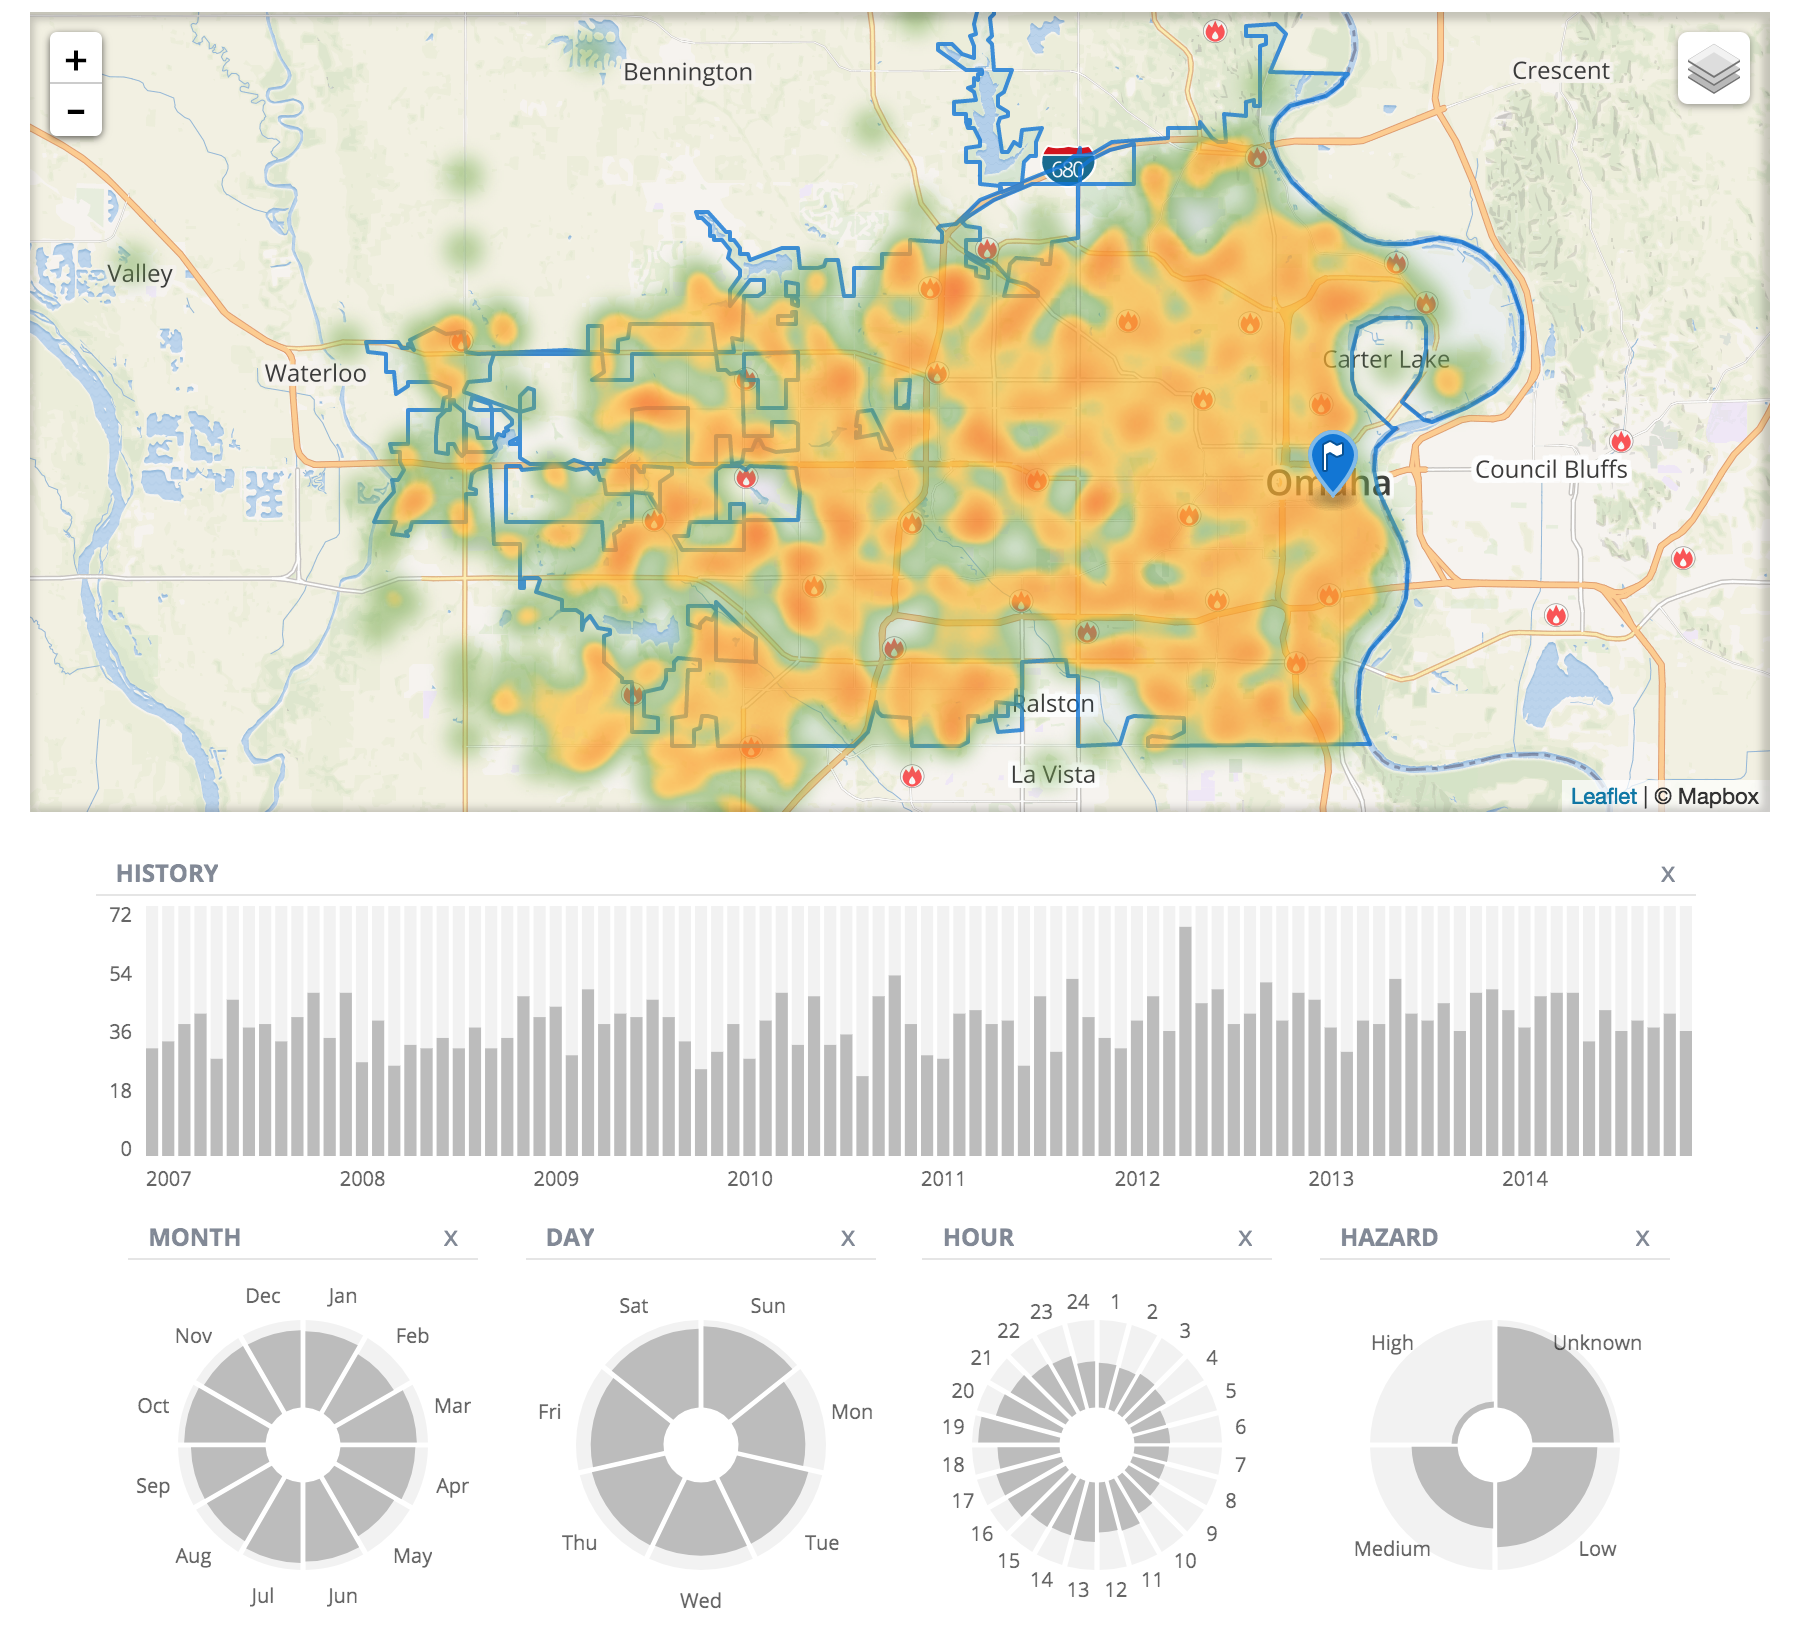
\includegraphics[width=.9\columnwidth]{Figures/interactive_fire_map}
\caption{Interactive geospatial map of fires that is sortable by time and parcel hazard level.}
\label{fig:interactive_fire_map}
\end{figure}

Clicking on any of the features on the dashboard will filter the heat map data accordingly. Users can filter the data by time (month, year, hour) or by structure hazard level (low, medium, high, or unknown). Any of these filters can be applied at the same time. To remove a filter, click the respective `x' icon nearest the applied filter. The filters include history, month, day, hour, and hazard.

\FloatBarrier

\section{Interactive Parcel Data}

Data specific to each parcel within the community are provided by hovering over the stack of paper icon in the upper right corner of the map and clicking on the `Parcels' radio button. To view the parcels, please zoom in on the map 4 levels. If the parcels do not show up right away, allow a moment for the data to load. Parcels are color coded by hazard level: green = low, orange = medium, and red= high. If you uncheck the `Jurisdiction Boundary' radio button, then you can click on any parcel and any of the known parcel attributes will appear. Figure~\ref{fig:parcel_data} shows an example of a department map with the parcel data loaded.

\begin{figure}[ht!]
\centering
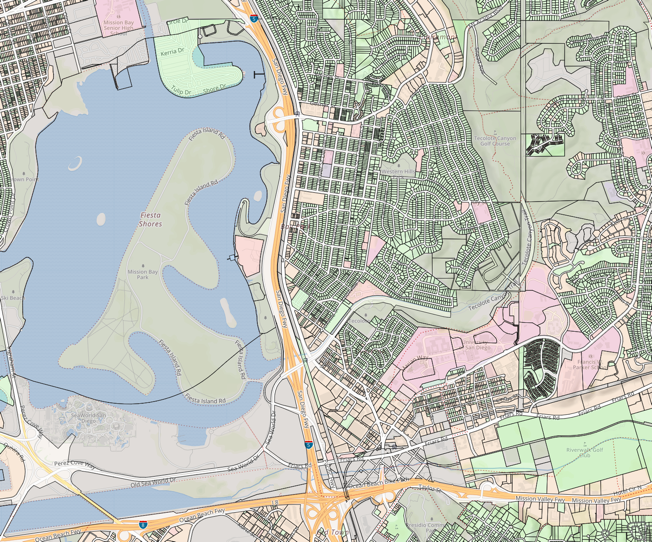
\includegraphics[width=.9\columnwidth]{Figures/parcel_data}
\caption{Interactive map showing hazard level of parcels as well as parcel specific information such as age, footprint, number of floors.}
\label{fig:parcel_data}
\end{figure}

\FloatBarrier

\section{Predicted Fire Estimates}

Using historical fire data (NFIRS) and characteristics about your community (community risk), estimates can be made regarding the number of fires, how big those fires may be, and the number of casualties. Figure~\ref{fig:fire_predictions} shows an example dialog box of these predictions.

\begin{figure}[ht!]
\centering
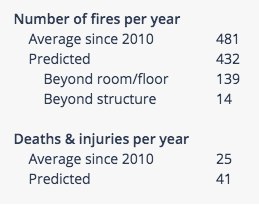
\includegraphics[width=.5\columnwidth]{Figures/fire_predictions}
\caption{Estimated prediction of number of fires, fire size, and number of causalities.}
\label{fig:fire_predictions}
\end{figure}

\chapter{Checking Your Department's Data}

Ensure that your department has the most accurate data.

\begin{enumerate}
\item Check the jurisdiction border. Please send an email to: \href{mailto:boundaries@firecares.org}{Contact Us: Boundaries}. Be sure to include your Fire Department Name and FDID as it is specified on \href{https://www.FireCARES.org}{FireCARES.org}. The map will be used to update your border.

\item Check your fire station list and corresponding addresses. If the station list on your department's page is incorrect, Please send an email to: \href{mailto:stations@firecares.org}{Contact Us: Stations}. Be sure to include your Fire Department Name and FDID as it is specified on \href{https://www.FireCARES.org}{FireCARES.org}.

\item Station Apparatus and Staffing Tables. Department Administrators/Users have necessary permissions to add data in the station apparatus and staffing tables to assure that your data are available for new GIS calculation features being implemented. 

\item Fire Data as a source of information. NFIRS data were used as the national source of fire incidents. For each department, the available NFIRS data were loaded and analyzed in the system.  As you can see the most recent data available at the national level are two years old. Departments may send NFIRS transaction files directly to FireCARES for loading to assure that all scores using attributes from this data are up to date.  

\end{enumerate}

Connect FireCARES to your NFORS data. As departments link to NFORS data modules, their data are not only real time for NFORS analytics but can also be used to populate the FireCARES system for real time feature updates. Go to \href{https://nfors.org}{NFORS.org} for more information on how to access NFORS module at no costs.

\chapter{Project Partners}

This work has been funded by DHS/FEMA's Assistance to Firefighter's Grant program. The work is a collaboration among several organizations to make FireCARES a tool for the fire service. The organizations are listed below:

\begin{itemize}
\item Commission on Fire Accreditation International (CFAI-Risk)
\item International Association of Fire Fighters (IAFF)
\item Underwriters Laboratories Firefighter Safety Research Institute (ULFSRI)
\item National Institute of Standards and Technology (NIST)
\item Urban Institute
\item The University of Texas at Austin
\item International Association of Fire Chiefs (IAFC)
\item Metropolitan Fire Chiefs
\end{itemize}

Other organizations that have helped with this project include Worcester Polytechnic University (WPI).

\chapter{List of Abbreviations}

\begin{tabbing}
\hspace{1.5in} \= \\

DHS \> Department of Homeland Security \\
ERF \> Effective response force \\
FDID \> Fire Department ID \\
FEMA \> Federal Emergency Management Agency \\
GIS \>  Geographic information system \\
IAFC \> International Association of Fire Chiefs \\
IAFF \> International Association of Fire Fighters \\
UL FSRI \> UL Firefighter Safety Research Institute \\
NIST \> National Institute of Standards and Technology  \\
NFIRS \> National Fire Incident Reporting System \\
\end{tabbing}

\bibliography{firecares}

\chapter*{Notes}

\end{document}
